\section{Results}
\subsection{Testing StabilityChecker: The Gardner toggle switch}

This toggle switch model was developed by T.~S. Gardner~\autocite{Gardner:2000vha}. This model consists of two mutually repressing transcription factors and is defined by the following ODEs:

\begin{align}
\frac{du}{dt} &= \frac{a_1}{1+v^{\beta}} - u \label{eq:gard_1} \\
\frac{dv}{dt} &= \frac{a_2}{1+u^{\gamma }} - v\label{eq:gard_2}
\end{align}
Where $a_1$ and $a_2$ are the effective rates of synthesis of repressors 1 and 2 respectively. \textit{u} is the concentration of repressor 1 and \textit{v} the concentration of repressor 2. \textit{$\beta$} is the cooperativity of repression of promoter 1 and \textit{$\gamma$} of repressor 2. In their paper,  T.~S. Gardner~\autocite{Gardner:2000vha} state that there are two conditions for bistability of this toggle switch model. That $a_1$ and $a_2$ are balanced and that $\beta$ and $\gamma$ are \textgreater 1. In order to test our methodology, we used StabilityChecker to find the posterior distribution for which this model exhibits bistable behaviour. So setting the desired behaviour to bistable, and using for priors a wide range of values that includes the values used in the Gardner paper, we test StabilityChecker to see if it finds the same conditions as the ones set by T.~S. Gardner. The prior distributions used are shown in Table~\ref{tab:gard}. The posterior distribution calculated by StabilityChecker is shown in Figure~\ref{fig:Gard_post}.

\begin{figure}[p]
\centering
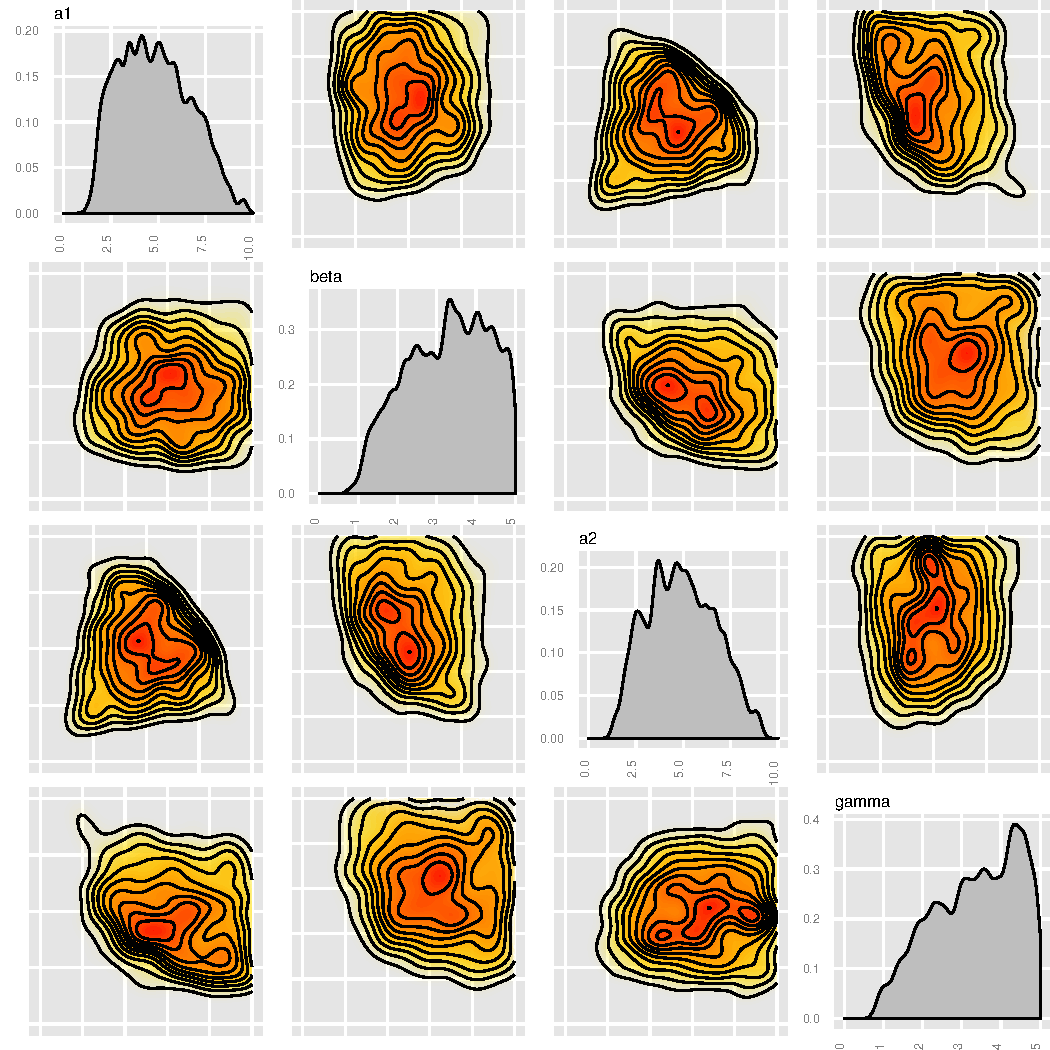
\includegraphics[scale=0.7]{chapterModelling/images/Gardner/posterior.pdf}
\caption[The posterior distribution of the bistable Gardner toggle switch]{The posterior distribution of the bistable Gardner toggle switch. The parameters $a_1$, $a_2$ represent to the effective synthesis rate of repressors 1 and 2 respectively. Parameters $\beta$, $\gamma$ represent the cooperativity on repressors 1 and 2 respectively. The marginal distributions of each parameter are found on the diagonal and pairwise joint distributions along the sides.}
\label{fig:Gard_post}
\end{figure}

\clearpage
\begin{figure}[p]
\centering
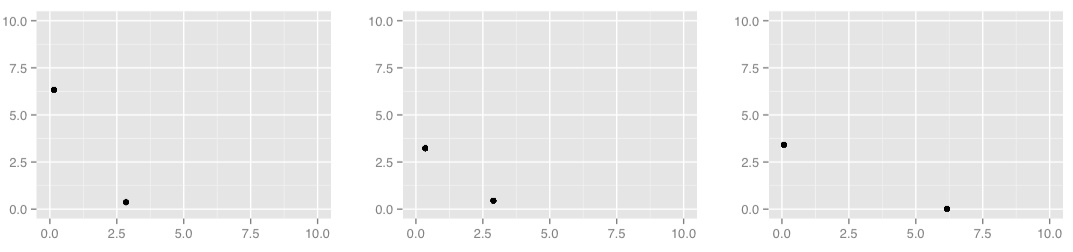
\includegraphics[scale=0.4]{chapterModelling/images/Gardner/phase_plots.png}
\caption{A sample of the phase plots produced from the final population of the Gardner switch.}
\label{fig:det_gard_phase}
\end{figure}

\begin{table}[p]
\centering
\caption{Gardner switch priors}
\label{tab:gard}
\begin{tabular}{cccc|cc}
\multicolumn{4}{c|}{Parameters} & \multicolumn{2}{c}{Species} \\ %\hline
$a_1$   & $\beta$   & $a_2$   & $\gamma$  &   $s_1$      &       $s_2$   \\
0-10    & 0-5       & 0-10    &  0-5      &      0-100   &          0-100   
\end{tabular}
\end{table}

These results agree with the results reported by the original paper~\autocite{Gardner:2000vha} . For this switch to be bistable $a_1$ and $a_2$ must be balanced while $\beta$ and $\gamma$ must both be \textgreater 1, as can be seen in the marginal distributions of $\beta$ and $\gamma$ in Figure~\ref{fig:Gard_post}. The conditions set by the original paper for parameters $a_1$ and $a_2$ are met, as the joint distribution shown in Figure~\ref{fig:Gard_post} matches the bifurcation lines calculated in the original paper. 
This successful test demonstrates that StabilityChecker can be used to find the stability a model is capable of as well as the parameter ranges that can produce that. This allows us to confidently apply the methodology to further models.
%-%-%-%-%-%-%%-%-%-%-%-%-%%-%-%-%-%-%-%
\newpage
\subsubsection{Comparing the deterministic and stochastic cases} 
    
There are two main ways of modelling a system, deterministically and stochastically. Deterministic modelling utilises ordinary differential equations (ODE) and models the concentrations of the species (proteins or other molecules) by time-dependent variables~\autocite{deJong:2002ft}. Rate equations are used to model gene regulation where the rate of production of a species is a function of the concentrations of the other species~\autocite{deJong:2002ft}. When modelling deterministically the model is viewed as a system which, with sufficient knowledge of the system, its behaviour is entirely predictable. Nevertheless we are still a long way away from having complete knowledge of a system of interesting size~\autocite{wilkinson:2006}. Deterministic modelling also assumes a homogenous mixture where species concentrations vary continuously and deterministically, assumptions that often are not met \textit{in vivo}. A cell is spatially and temporally separated, due to small molecule numbers and fluctuations in the timing of processes~\autocite{deJong:2002ft}.  
   
In stochastic modelling, species are measured in discrete amounts rather than concentrations and a joint probability distribution is used to express the probability that at time \textit{t} the cell contains a number of molecules of each species~\autocite{deJong:2002ft}. It takes uncertainty into account and does not assume a homogenous mix. It is thus often more appropriate for modelling cellular systems, although more computationally intensive. In stochastic systems the Gillespie algorithm is widely used to simulate the time-evolution of the state of the system~\autocite{Warren:2005kea}.

The toggle switch has been modelled both deterministically and stochastically, with the two methods producing different results. Thus here we use StabilityChecker to compare the stabilities that the model is capable of, under the different simulation types. By using the same framework, and the same prior distributions for the models, one can directly compare the posterior distributions produced by the deterministic and the stochastic case, and uncover the effects that are due to the stochasticity of the system. This is relevant in a a biological model in which small molecule numbers and external noise are not negligible. Using StabilityChecker and using the same priors for the two models (Table~\ref{tab:gard_det_stoch}), we calculated the posterior for each both bistable models. The results are shown in Figures~\ref{fig:Gard_post_det_high},~\ref{fig:Gard_post_stch}. The prior ranges used are much wider than in the test case in order to allow more flexibility in both models and have a greater range over which to compare the models. 

\clearpage
\begin{table}[p]
\centering
\caption{Gardner switch priors}
\label{tab:gard_det_stoch}
\begin{tabular}{cccc|cc}
\multicolumn{4}{c|}{Parameters} & \multicolumn{2}{c}{Species} \\ %\hline
$a_1$   & $\beta$   & $a_2$   & $\gamma$  &   $s_1$      &       $s_2$   \\
0-60    & 0-5       & 0-60    &  0-5      &      0-100   &          0-100   
\end{tabular}
\end{table}


\begin{figure}[p]
\centering
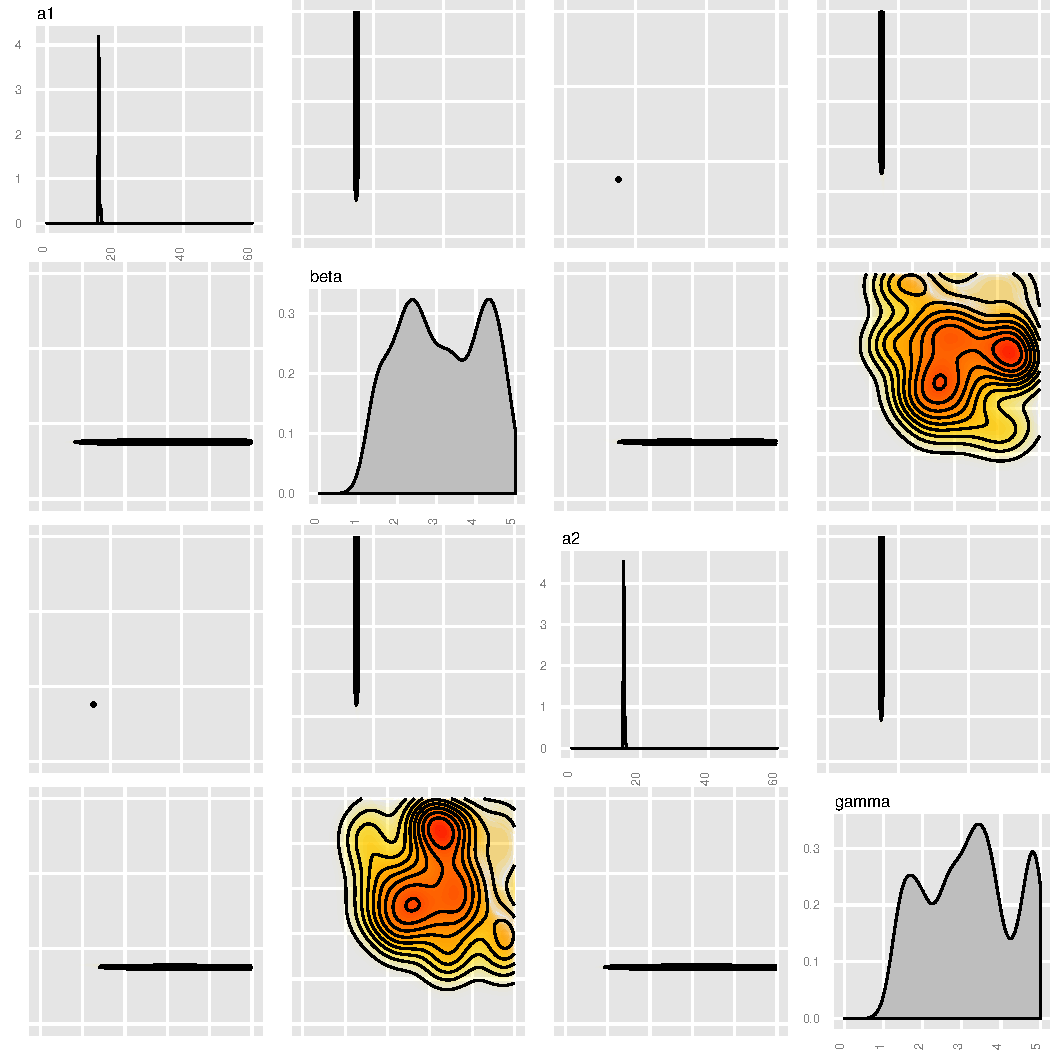
\includegraphics[scale=0.7 ]{chapterModelling/images/Gardner/posterior_det_high_mean.pdf}
\caption{The posterior distribution of the deterministic model of the Gardner toggle switch.}
\label{fig:Gard_post_det_high}
\end{figure}
\newpage

\begin{figure}[p]
\centering
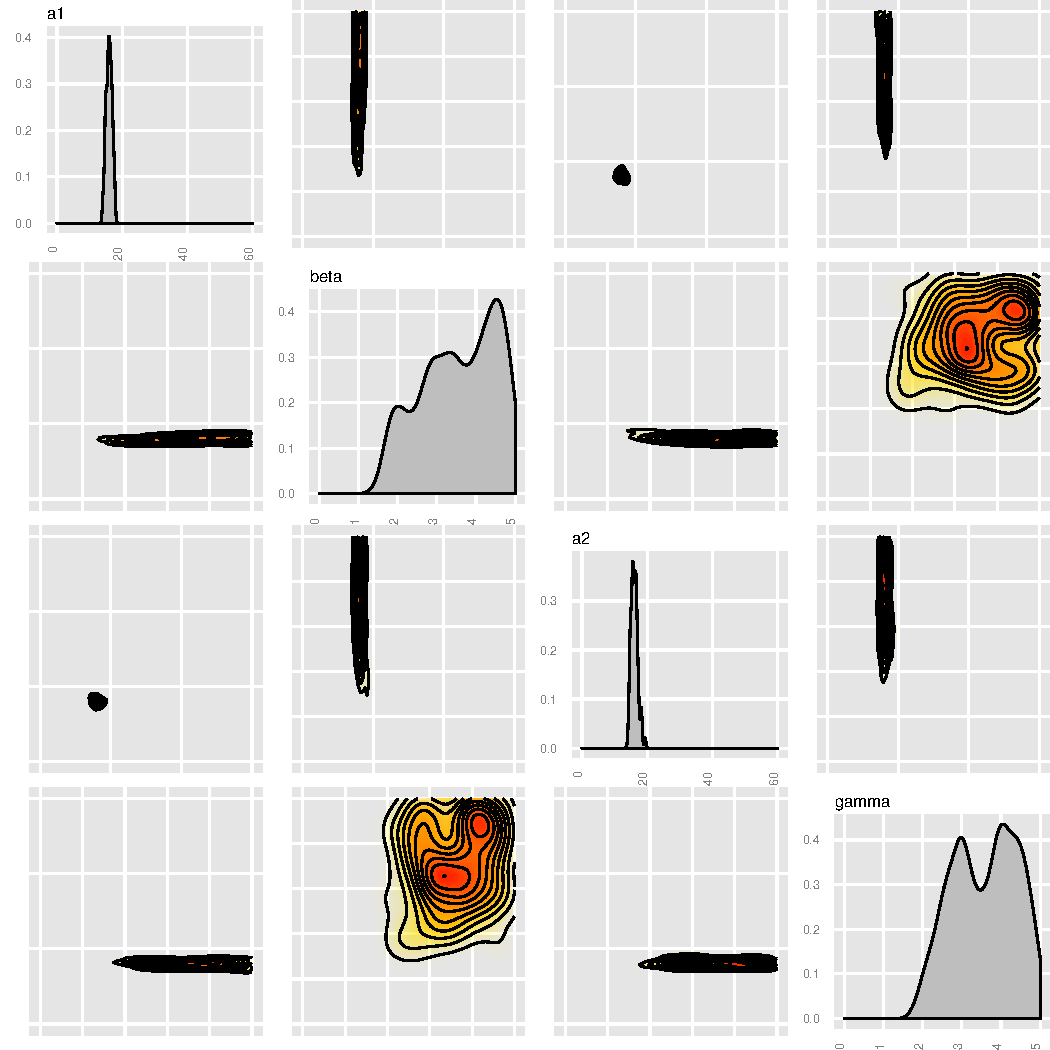
\includegraphics[scale=0.7]{chapterModelling/images/Gardner/posterior_stch_high_mean.pdf}
\caption{The posterior distribution of the stochastic model of the Gardner toggle switch.}
\label{fig:Gard_post_stch}
\end{figure}

As can be seen in the above results, stochasticity has a big effect on the posterior. Firstly, a greater parameter range can produce a bistable behaviour when stochastic effects are taken into account. The condition set by T.~S Gardner~\autocite{Gardner:2000vha} for the values of $a_1$ and $a_2$ to be balanced holds in both the deterministic and stochastic cases but in the stochastic case this is met by a wider range of values. The second conditions of $\beta$  and $\gamma$ \textgreater 1 also needs to be met in the stochastic case. 

\begin{figure}[p]
\centering
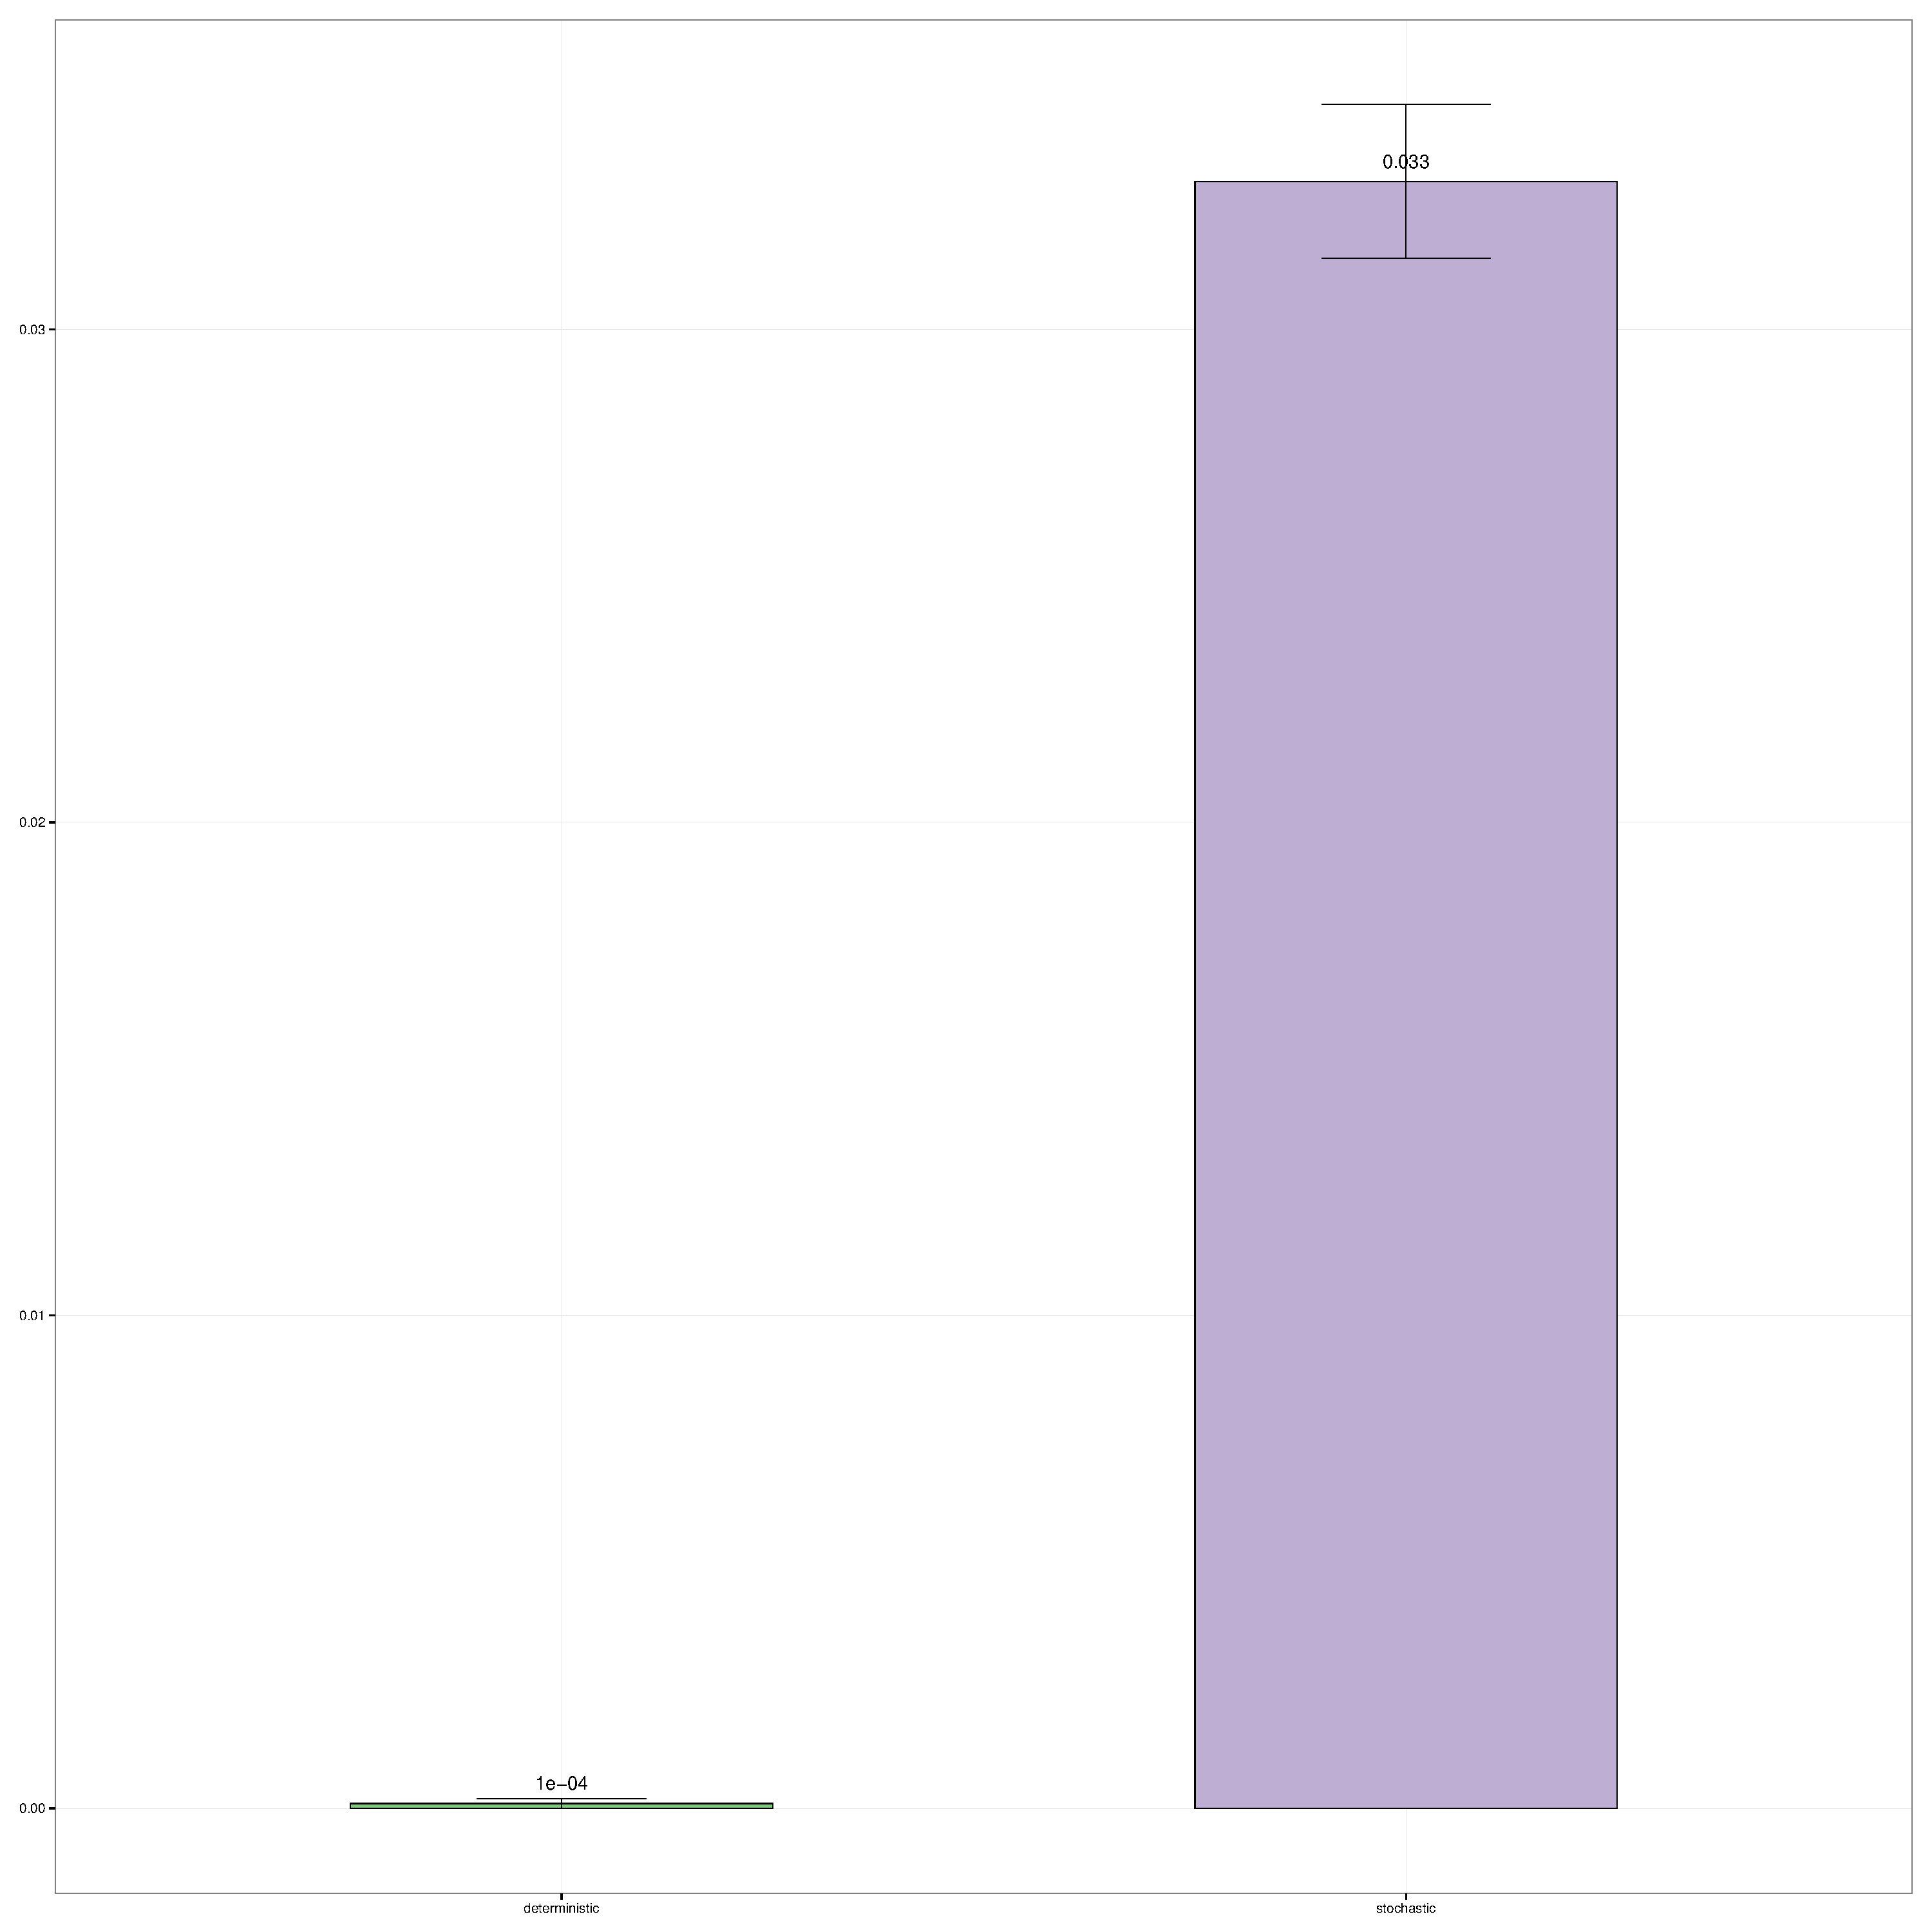
\includegraphics[scale=0.2]{chapterModelling/images/Gardner/robustness_comparison_high_mean.pdf}
\caption{Comparing the robustness of the deterministic and stochastic Gardner switch models}
\label{fig:Gard_robst}
\end{figure}

 When stochasticity is taken into account, robustness increases significantly as seen in Figure~\ref{fig:Gard_robst}. This indicates that stochasticity increases the ability of the model to withstand fluctuations in parameter values and still produce the desired bistability. A deterministic model cannot predict this increased robustness.


%-%-%-%-%-%-%-%-%-%-%-%-%-%-%-%-%-%-%-%-%-%-%-%-%-%-%-%-%-%-%-%-%-%-%-%-%-%-%-%-%-%-%-%-%-%-%-%-%-%
\newpage
\section{Lu toggle switch models}

In their study, \textcite{Lu:2013br} explored the effect of white Gaussian and shot noise on the multi-state switches. They found that the classical toggle switch, with the repressing transcription factors has two steady states and the toggle switch with added double positive auto-regulation has three steady states. By extending the analysis on these models by using StabilityChecker we can determine the design principles that make a tristable versus a bistable switch. This is another example of a use for StabilityChecker.
The system used in their study is defined by two dynamical systems:

\begin{align}
\dot{x} &= f_{x}(x,y) =g_{x}\, H^{S}_{xy}(y)\, H^{S}_{xx}\,(x)-k_{x}x \label{eq:lu_both_1} \\
\dot{y} &= f_{y}(x,y) =g_{y}\,H^{S}_{yx}(x)\,H^{S}_{yy}\,(y)-k_{y}y \label{eq:lu_both_2}
\end{align}
\begin{align}
H^{S}_{xx} &= H^{-}_{x}(x)+\lambda_{x}H^{+}_{x}(x)\label{eq:lu_hsxx}\\
H^{-}_{x}(x) &= 1 \big/\left[1+(x/a_{x})^{n_{x}}\right]\label{eq:lu_hpx}\\
H^{+}_{x}(x) &= 1-H^{-}_{x}(x)\label{eq:lu_hmx}
\end{align}
%\begin{align*}%
%	\left\{S^3_\text{this} \frac{1}{2}\right.
%\end{align*}

For the classical model, in which no self-activation is present, the system reduces to the following equations:

\begin{align}
\dot{x}=f_{x}(x,y) &= g_{x}H^{S}_{xy}(y)-k_{x}x,\label{eq:lu_cl_1}\\
\dot{y}=f_{y}(x,y) &= g_{y}H^{S}_{yx}(x)-k_{y}y\label{eq:lu_cl_2}
\end{align}
For the parameter values used in the Lu study, as shown in Table ~\ref{tab:lu_cl_bi}, the system exhibits three positive steady states (Figure ~\ref{fig:lu_bis_class}), of which two are stable and one is unstable. 

\clearpage
\begin{figure}[p]
\centering
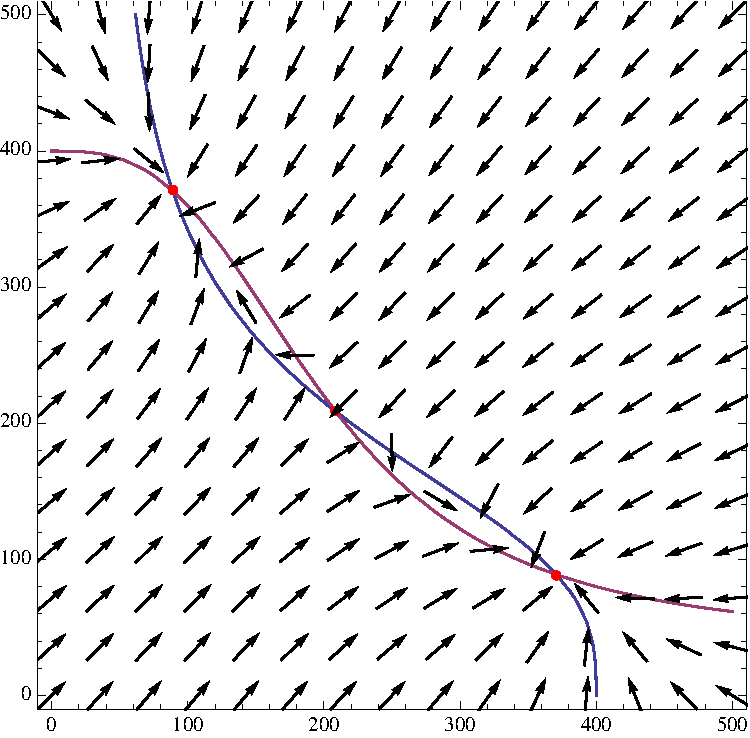
\includegraphics[scale=0.7]{chapterModelling/images/Lu/mae/classic.pdf}
\caption[Phase portrait of the Lu classical model with no self activation]{Phase portrait of the Lu classical model with no self activation. There are two stable steady states and one unstable steady state.}
\label{fig:lu_bis_class}
\end{figure}

\begin{table}[p]
\centering
\caption{Lu classical model parameter values}
\label{tab:lu_cl_bi}
\begin{tabular}{cccccccccc}
gx    & gy    & kx    & ky    & nxy & nyx & xxy     & xyx     & Ixy   & Iyx \\
40&40     &0.1   & 0.1   &  3  &  3  &  200    &  200    & 0.1    &   0.1
\end{tabular}
\end{table}

Using StabilityChecker with priors centred around the parameter values used in the original paper (Table ~\ref{tab:lu}), we can find the robustness of this bistable behaviour, as well as identify the most important parameters for bistability. The posterior distribution of this model is shown in Figure ~\ref{fig:lu_bistable}. As can be seen from the posterior, the most restrained parameters are kx and ky, the parameters responsible for the degradation of the species involved. This indicates that the rate of degradation of the species is critical for the desired dynamic to occur. 

\begin{figure}[p]
\centering
\includegraphics[scale=0.8]{chapterModelling/images/Lu/posterior_100p_narrow.pdf}
\caption[The posterior distribution of the Lu classical model with no self activation]{The posterior distribution of the Lu classical model with no self activation. kx and ky are the most constrained parameters.}
\label{fig:lu_bistable}
\end{figure}


\clearpage
\begin{figure}[p]
\centering
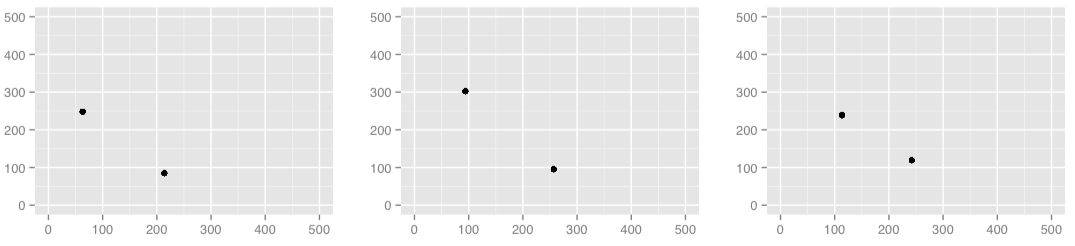
\includegraphics[scale=0.4]{chapterModelling/images/Lu/phase_plot.png}
\caption{A sample of the phase plots produced from the final population of the Lu classical model.}
\label{fig:lu_phase}
\end{figure}

\begin{table}[p]
\centering
\caption{Lu classical model priors}
\label{tab:lu}
\begin{tabular}{cccccccccc}
gx    & gy    & kx    & ky    & nxy & nyx & xxy     & xyx     & Ixy   & Iyx \\
35-45 & 35-45 & 0-0.2 & 0-0.2 & 2-4 & 2-4 & 150-250 & 150-250 & 0-0.2 &   0-0.2 
\end{tabular}
\end{table}

If self-activation is included, then the system is that presented in equations \eqref{eq:lu_both_1, eq:lu_both_2} . When values that are presented in table 1 are assigned to the parameters for the self-activating model, the system exhibits five positive steady states~\ref{fig:lu_tri_phse}. 

\clearpage
\begin{table}[p]
\centering
\caption{Lu model with self-activation parameter values}
\label{tab:lu_dp_tri}
\begin{tabular}{cccccccccc}
gx    & gy    & kx    & ky    & nxy & nyx & xxy     & xyx     & Ixy   & Iyx \\
4&4     &0.1   & 0.1   &  1  &  1  &  200    &  200    & 0.1    &   0.1
\end{tabular}
\end{table}

\begin{figure}[p]
\centering
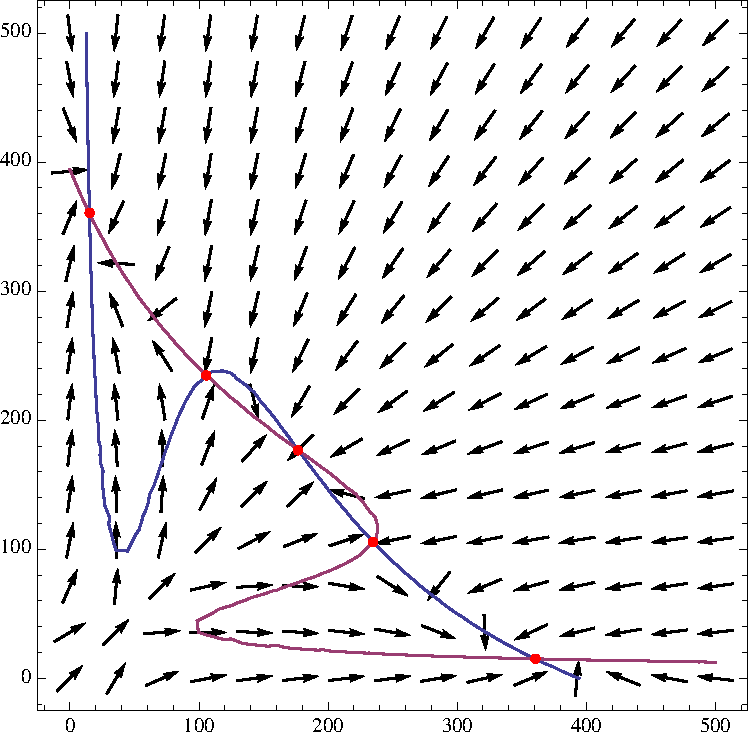
\includegraphics[scale=0.7]{chapterModelling/images/Lu/mae/selfactivation.pdf}
\caption[Phase portrait of the Lu model including double self-activation]{Phase portrait of the Lu model including double self-activation. The model had three stable steady states and two unstable steady states.}
\label{fig:lu_tri_phse}
\end{figure}

Using StabilityChecker and priors centred around the original values, shown in Table~\ref{tab:lu_dp_pr}, we can explore the robustness of this behaviour, in a similar way as done for the classical model. The posterior is shown in Figure~\ref{fig:lu_tristable}. The most constrained parameters are kx and ky, similar as in the classic toggle switch case.

\clearpage
\begin{table}[p]
\centering
\caption{Lu model with double self-activation priors}
\label{tab:lu_dp_pr}
\begin{tabular}{cccccccccc}
gx    & gy    & kx    & ky    & nxy & nyx & xxy     & xyx     & Ixy   & Iyx \\
3-5 & 3-5 & 0-0.2 & 0-0.2 & 0-2 & 0-2 & 150-250 & 150-250 & 0-0.2 &   0-0.2 
\end{tabular}
\end{table}

\begin{figure}[p]
\centering
\includegraphics[scale=0.3]{chapterModelling/images/Lu/tri/posterior_1000p_1.pdf}
\caption[The posterior distribution of the Lu model with double self activation]{The posterior distribution of the Lu model with double self activation. kx and ky are the most constrained parameters.}
\label{fig:lu_tristable}
\end{figure}


\begin{figure}[p]
\centering
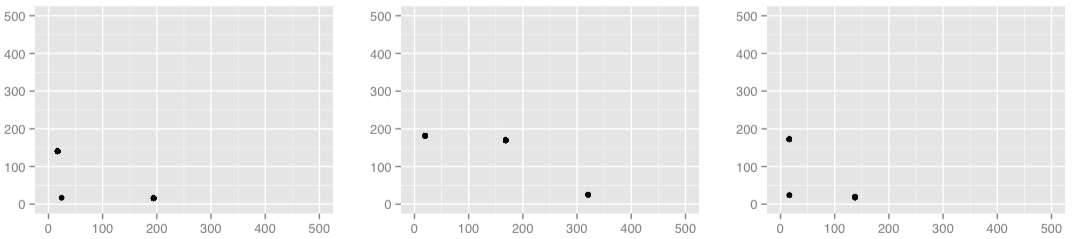
\includegraphics[scale=0.4]{chapterModelling/images/Lu/tri/phase_plots.png}
\caption{A sample of the phase plots produced from the final population of the Lu tristable model.}
\label{fig:lu_tri_phase_pl}
\end{figure}


\subsubsection{Extracting switch design principles}
Next, we went on to study the design principles that make a switch tristable vs bistable. To do this we implemented an algorithm, as shown in the Appendix. Samples were taken from posterior distribution of the Lu tristable switch. Then we separate the values, for each parameter, that were also found in the posterior of the bistable switch. The same procedure was done but taking samples from the bistable posterior and looking for them in the tristable posterior. This can give an indication of the separation of parameter values that can give rise to a bistable vs a tristable switch. 

The results are shown in Figure ~\ref{fig:lu_bi_tri}.
\clearpage
\begin{figure}[p]
\centering
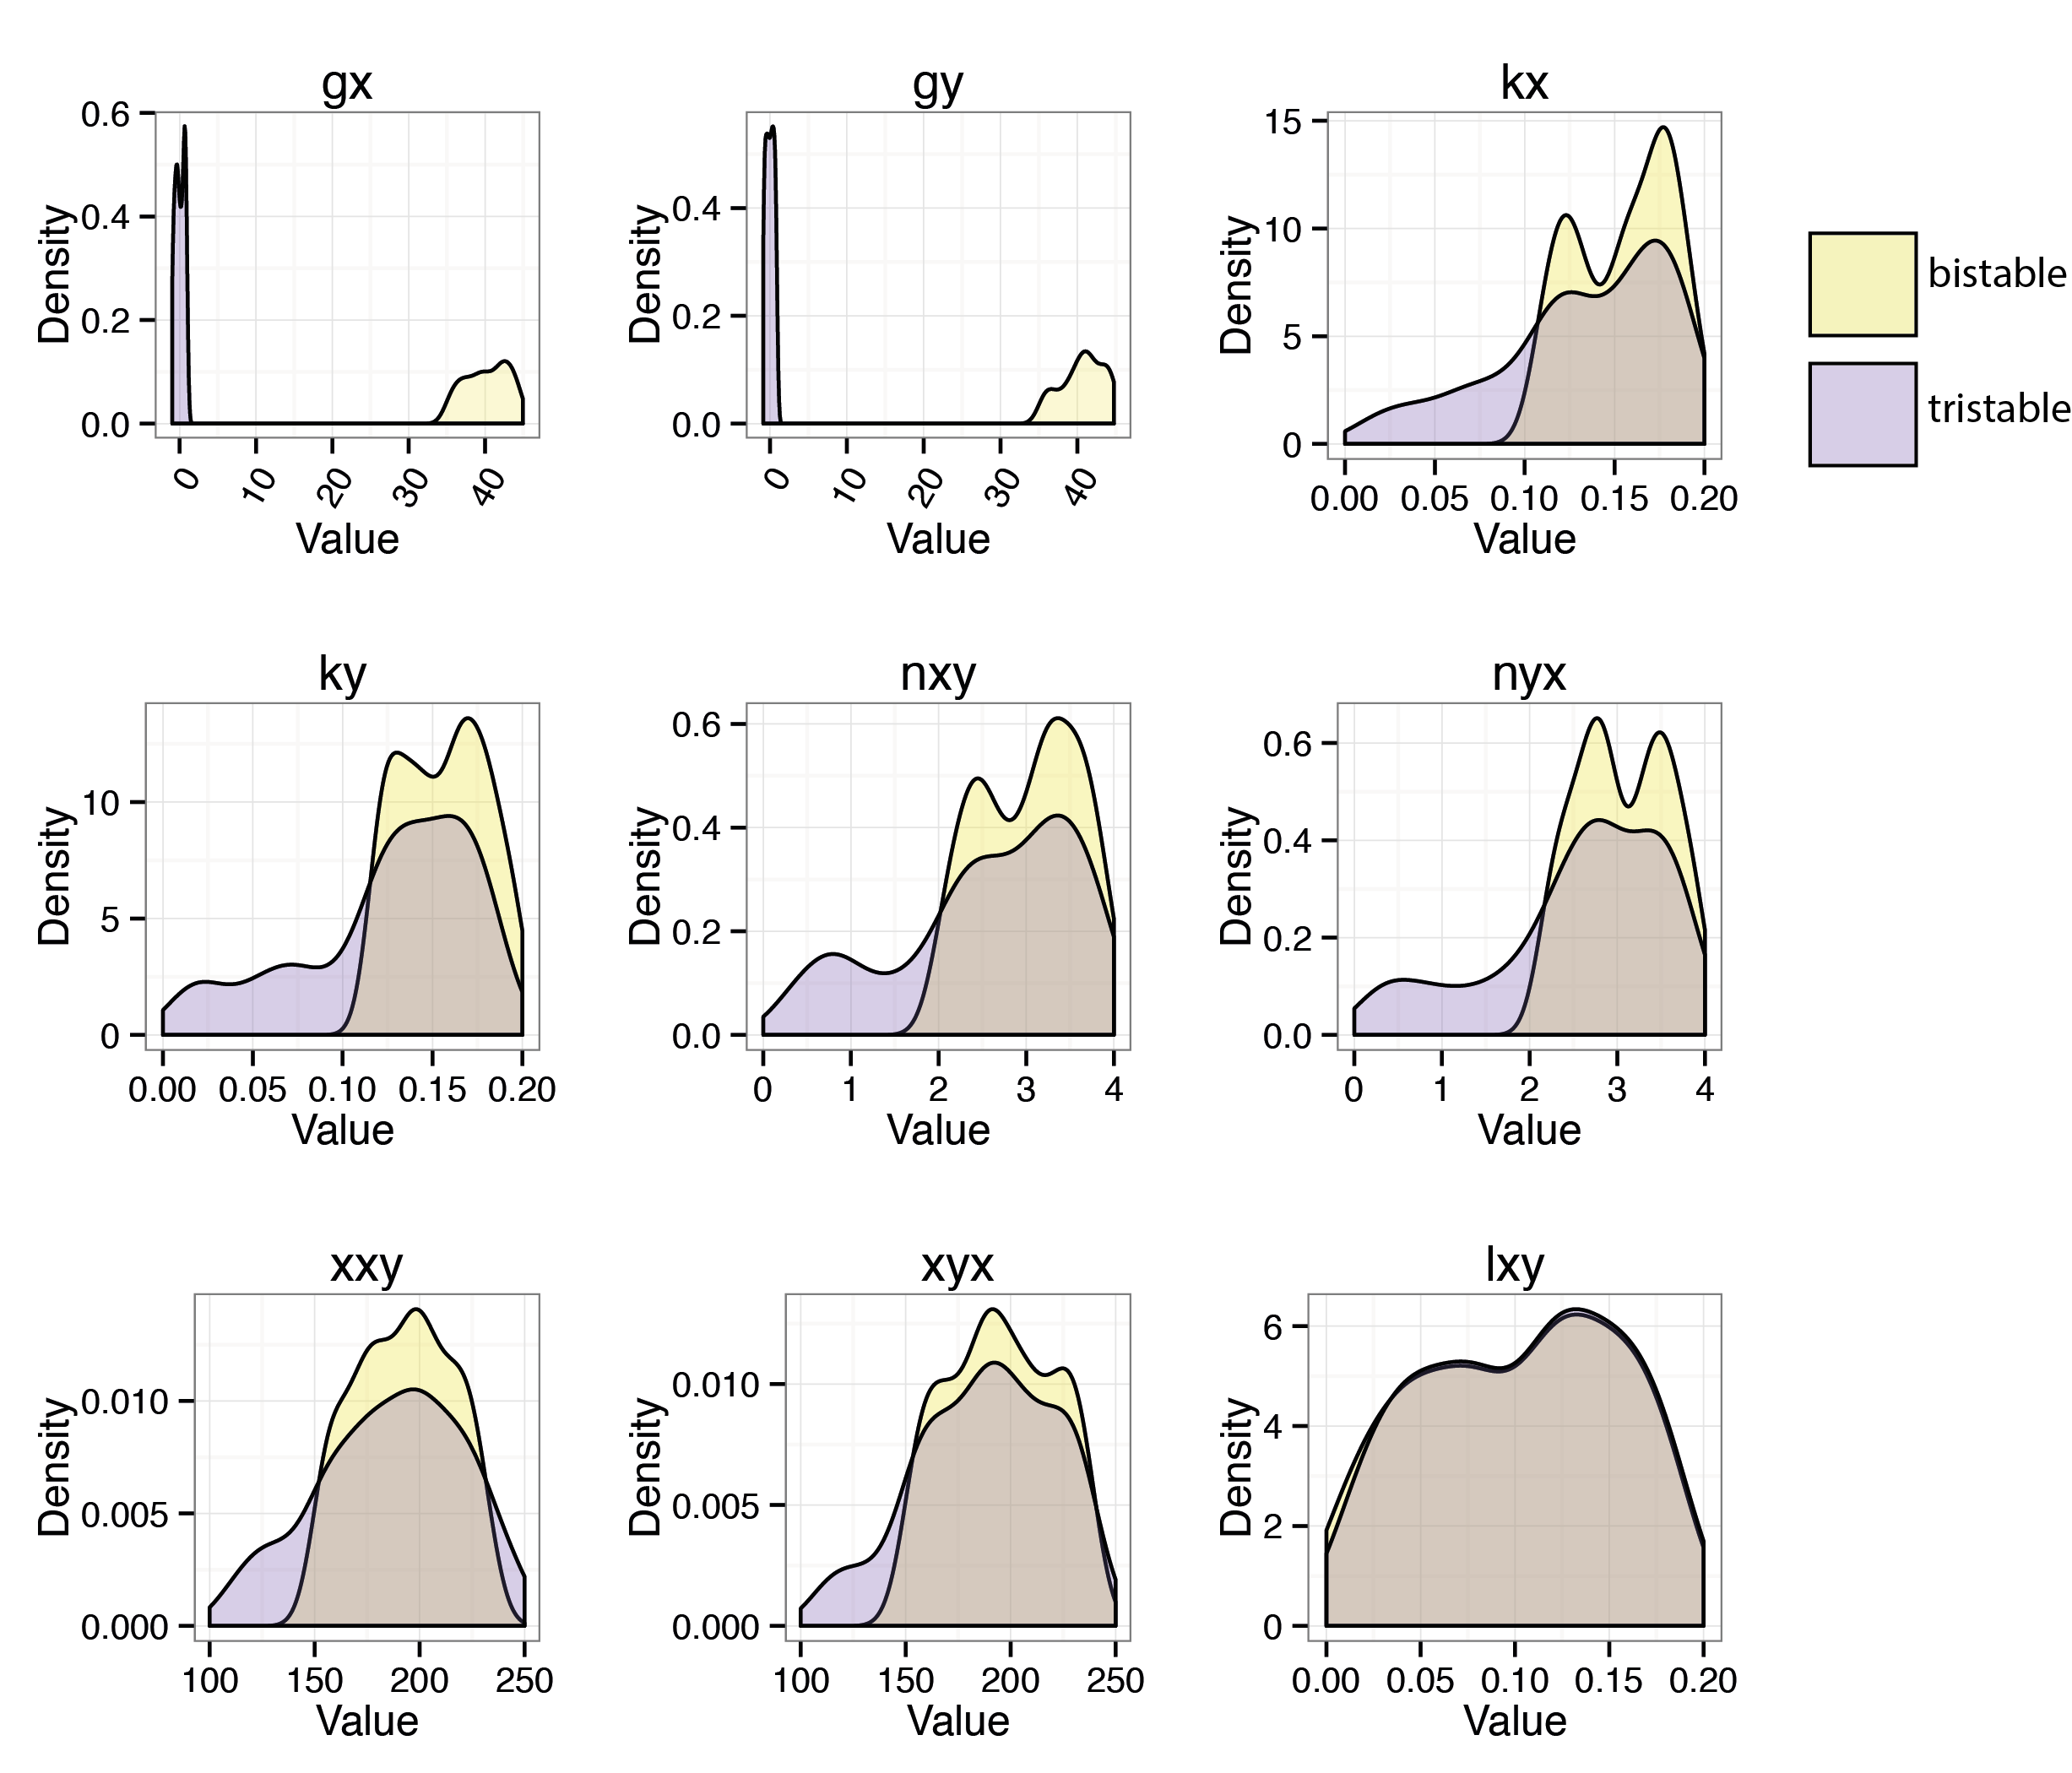
\includegraphics[scale=0.8]{chapterModelling/images/design_principles/res_all_tri_biyp.png}
\caption{Extracting the tristable versus bistable switch design principles}
\label{fig:lu_bi_tri}
\end{figure}

It is clear from the above results that the values for gx and gy are very different for producing a bistable versus a tristable switch. In order to further test this result, we used the model with self activation, with the same priors as used in the tristable case (Table~\ref{tab:lu_dp_tri}), except for the values of gx and gy, which we swapped for the values found to produce a bistable switch. This new model was then analysed using StabilityChecker and was found to be bistable. This indicates that the values of gx and gy, representing gene expression, are critical for the design of a switch with a given stability, and changing their values can make a tristable switch bistable. This can be seen in the phase plots produced, shown in Figure~\ref{fig:lu_bi_tri}

\begin{figure}[p]
\centering
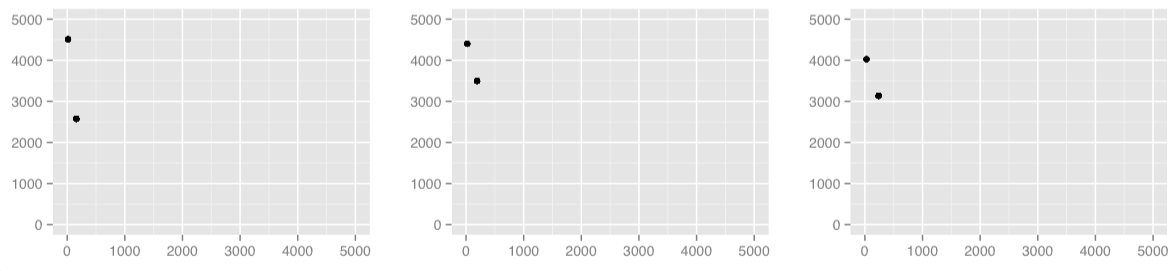
\includegraphics[scale=0.4]{chapterModelling/images/Lu/tri/phase_plot_tri_bi.png}
\caption{The phase plots produced by the last population of StabilityChecker. By changing only the parameters gx and gy in the Lu model with self-activation, the switch became a bistable switch, instead of a tristable switch.}
\label{fig:lu_bi_tri}
\end{figure}


%-%-%-%-%-%-%-%-%-%-%-%-%-%-%-%-%-%-%-%-%-%-%-%-%-%-%-%-%-%-%-%-%-%-%-%-%-%-%-%-%-%-%-%-%-%-%-%-%-%
\newpage
\subsection{Positive auto-regulation increases robustness to parameter fluctuations}

When faced with a set of competing designs for a given genetic circuit, one is likely to choose the simplest possible model that can achieve the desired behaviour. However, simple systems are often the least robust. Feedback loops are well known key regulatory motifs \autocite{Brandman:2005ci}. Negative feedback loops are essential for homeostasis and buffering \autocite{Thomas:1995id} thus increasing robustness to extrinsic noise sources and positive feedback loops can generate multistationarity in a system \autocite{Thomas:1995id}. Incorporating this kind of additional feedback interactions can make a design more robust and reliable. 

Building robust devices is critical for the success of synthetic biology. A robust device is a device that can withstand fluctuations in parameter values and still produce the desired behaviour. Here we use StabilityChecker to compare the robustness of two switches, a simple toggle switch and a switch with added positive auto-regulation. These models avoid the quasi-steady state approximation (QSSA) often used in modelling the toggle switch. Since StabilityChekcker is able to analyse models with numerous equations and parameters, there is no need for this assumption, which approximates a solution. Using Mass Action, the two models used are shown below:

Standard toggle switch:
$$
\begin{array}{cccc}
      \textrm{gA}\stackrel{\textrm{ge}}{\longrightarrow}\textrm{gA} + \textrm{A} \\
      \textrm{gB}\stackrel{\textrm{ge}}{\longrightarrow}\textrm{gB} + \textrm{B} \\
      \textrm{A} + \textrm{A} \stackrel{\textrm{dim}}{\longrightarrow}\textrm{A2} \\
      \textrm{A2} \stackrel{\textrm{dim r}}{\longrightarrow}\textrm{A} + \textrm{A} \\
      \textrm{B} + \textrm{B} \stackrel{\textrm{dim}}{\longrightarrow} \textrm{B2} \\
      \textrm{B2} \stackrel{\textrm{dim\_r}}{\longrightarrow}\textrm{B} + \textrm{B} \\
      \textrm{gA} + \textrm{B2} \stackrel{\textrm{rep}}{\longrightarrow}\textrm{B2gA} \\
      \textrm{B2gA} \stackrel{\textrm{rep\_r}}{\longrightarrow}\textrm{B} + \textrm{gA} \\
      \textrm{gB} + \textrm{A2} \stackrel{\textrm{rep}}{\longrightarrow}\textrm{A2gB} \\
      \textrm{A2gB} \stackrel{\textrm{rep\_r}}{\longrightarrow}\textrm{A2} + \textrm{gB} \\
      \textrm{A} \stackrel{\textrm{deg}}{\longrightarrow}\textrm{\O}\\
      \textrm{B} \stackrel{\textrm{deg}}{\longrightarrow}\textrm{\O}\\
      \textrm{S} + \textrm{A2} \stackrel{\textrm{rep\_dim}}{\longrightarrow}\textrm{SA2}\\
      \textrm{SA2} \stackrel{\textrm{rep\_dim\_r}}{\longrightarrow}\textrm{S} + \textrm{A2}\\
      \textrm{R} + \textrm{B2} \stackrel{\textrm{rep\_dim}}{\longrightarrow}\textrm{RB2}\\
      \textrm{RB2} \stackrel{\textrm{rep\_dim\_r}}{\longrightarrow}\textrm{R} + \textrm{B2}\\
      \textrm{R} \stackrel{\textrm{deg}}{\longrightarrow} \textrm{\O}\\
      \textrm{S} \stackrel{\textrm{deg}}{\longrightarrow}\textrm{\O}\\
\end{array}
$$

Double positive autoregulation:
$$
\begin{array}{cccc} 
    \textrm{A2} + \textrm{gA} \stackrel{\textrm{aut 1}}{\longrightarrow} \textrm{A2gA} \\
    \textrm{A2gA} \stackrel{\textrm{aut 2}}{\longrightarrow} \textrm{A} + \textrm{A2gA}\\
    \textrm{A2gA} \stackrel{\textrm{aut 3}}{\longrightarrow} \textrm{A2}+ \textrm{gA}  \\
    \textrm{B2} + \textrm{gB} \stackrel{\textrm{aut 1}}{\longrightarrow} \textrm{B2gB} \\
    \textrm{B2gB} \stackrel{\textrm{aut 2}}{\longrightarrow} \textrm{B} + \textrm{B2gB}\\
    \textrm{B2gB} \stackrel{\textrm{aut 3}}{\longrightarrow} \textrm{B2}+ \textrm{gB}  \\
\end{array}
$$

Using the same priors for their shared parameters, we used StabilityChecker for both models in order to compare their robustness. The corresponding posterioir distributions can be seen in Figures~\ref{fig:det_std} and ~\ref{fig:doub_pos}.

\clearpage
\begin{table}[p]
\centering
\caption{Mass Action switches priors}
\label{tab:simp}
\begin{tabular}{cccccccccc}
ge   & rep  & rep\_r & dim  & dim\_r & deg & deg\_dim & aut\_1 & aut\_2 & aut\_3\\
1-10 & 1-10 & 1-10    & 1-10 & 0-5    & 1-10 & 0-0.5   &1-10&5-10&1-5
\end{tabular}
\end{table}


\begin{figure}[p]
\centering
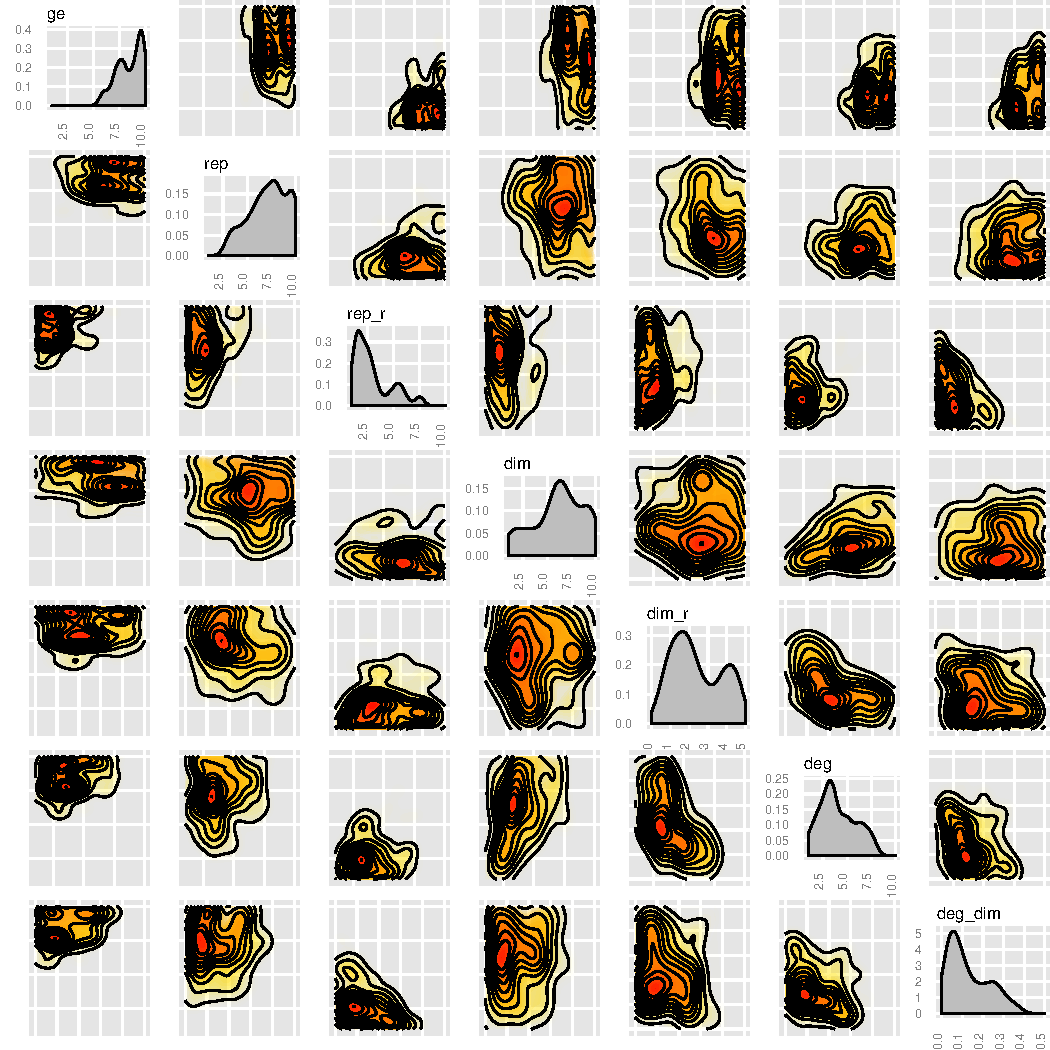
\includegraphics[scale=0.7]{chapterModelling/images/posterior_ma_cl_bi.pdf}
\caption{The posterior distribution of the mass action simple toggle switch}
\label{fig:det_std}
\end{figure}

\begin{figure}[p]
\centering
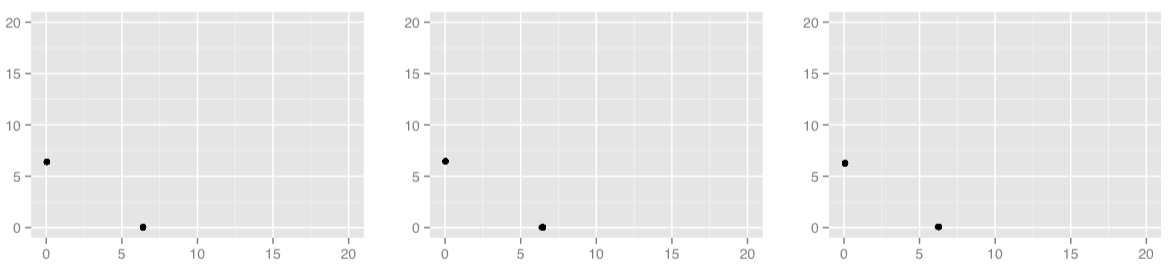
\includegraphics[scale=0.4]{chapterModelling/images/ma_cl_bi_phase_plot.png}
\caption{A sample of the phase plots produced from the final population of the mass action simple toggle switch.}
\label{fig:det_std_phase}
\end{figure}

\begin{figure}[p]
\centering
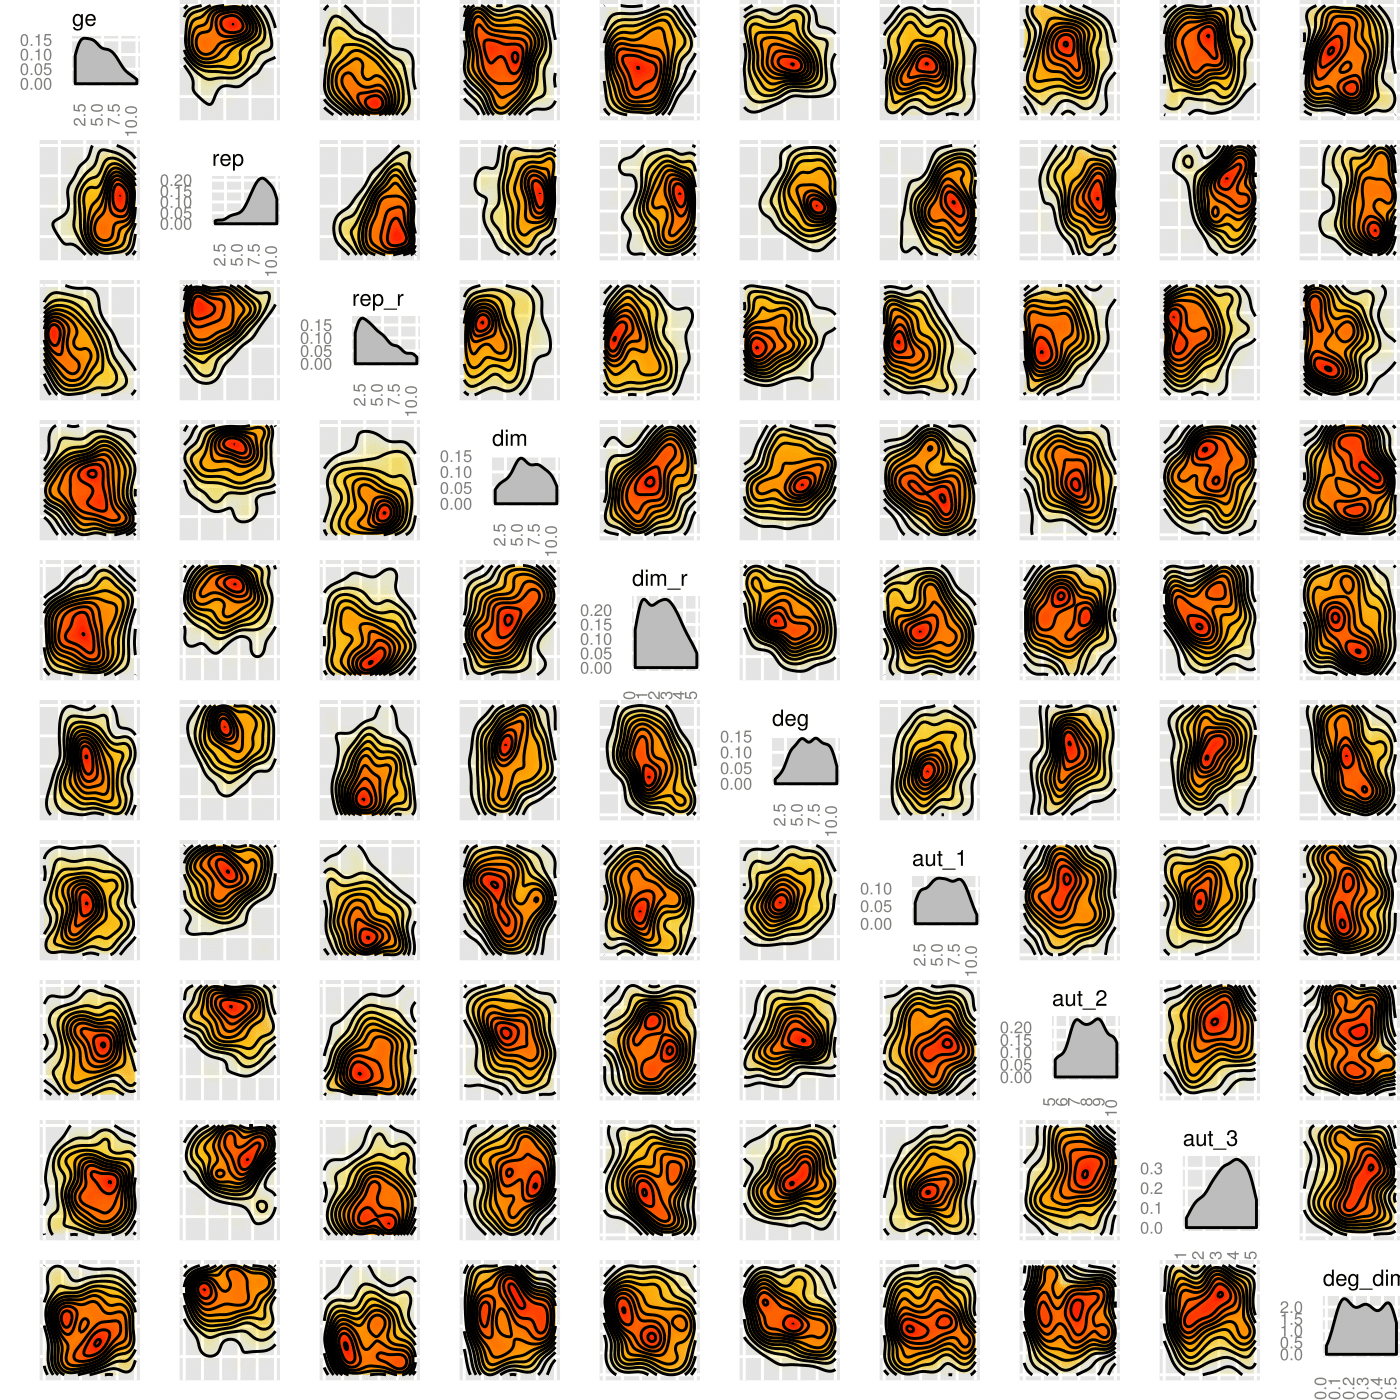
\includegraphics[scale=0.7]{chapterModelling/images/posterior_ma_dp_bi.pdf}
\caption{The posterior distribution of the Mass action double positive feedback loop switch}
\label{fig:doub_pos}
\end{figure}

\begin{figure}[p]
\centering
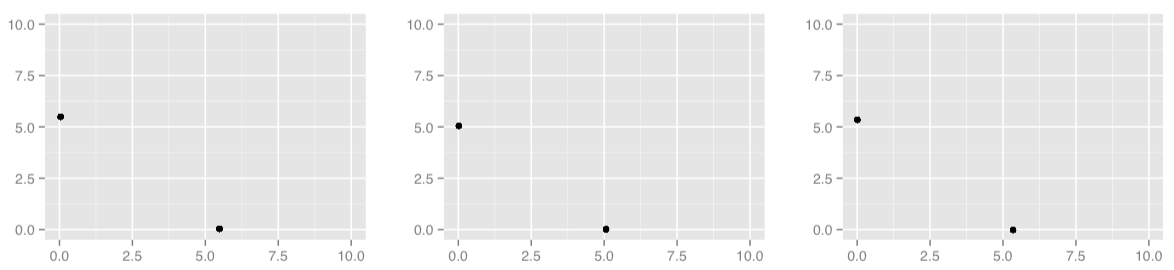
\includegraphics[scale=0.4]{chapterModelling/images/ma_dp_bi_phase_plot.png}
\caption{A sample of the phase plots produced from the final population of the mass action double positive feedback toggle switch.}
\label{fig:det_dp_phase}
\end{figure}

In order to directly compare the robustness of the two models, we used the algorithm outlined in the Methods as a measure of how wide each posterior is given the priors. The results are shown in Figure~\ref{fig:robust_std_doubpos}. 

\begin{figure}[p]
\centering
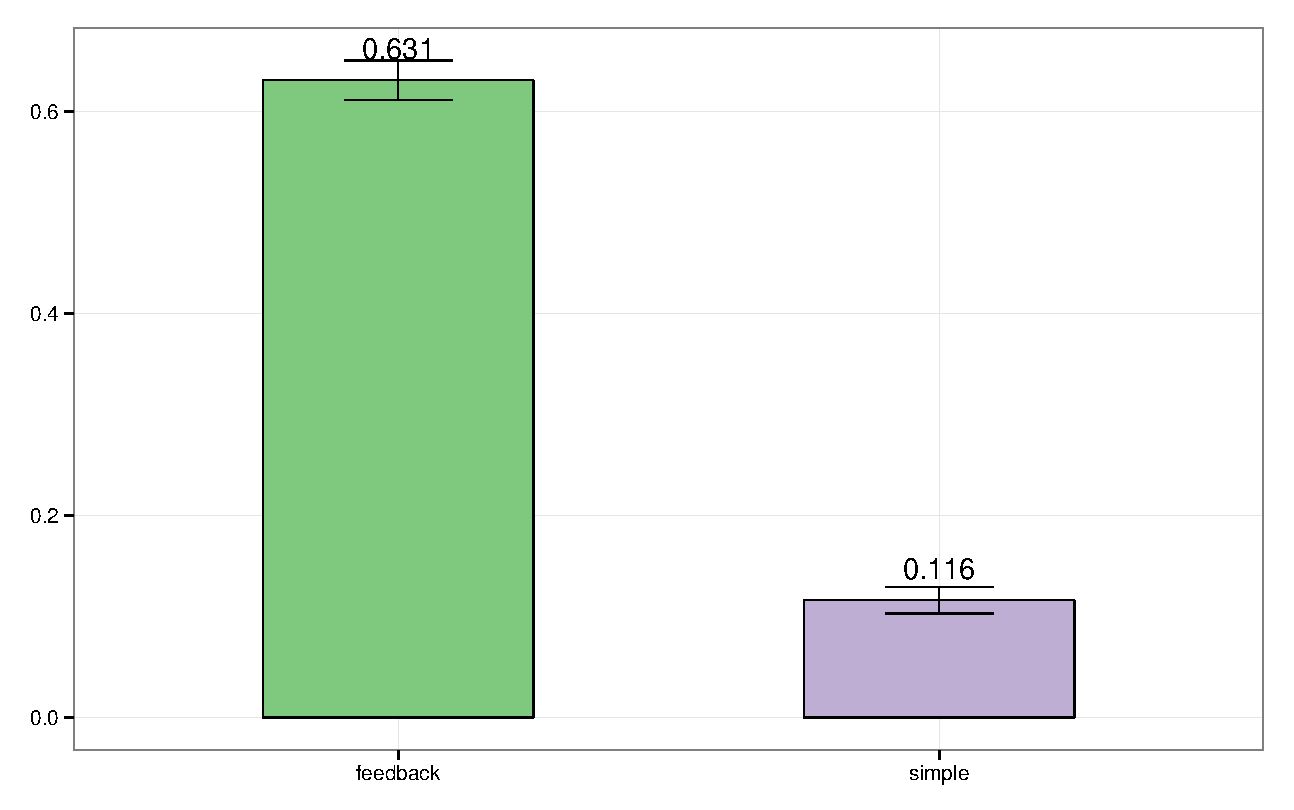
\includegraphics[scale=0.5]{chapterModelling/images/robustness_comparison.pdf}
\caption[The robustness of the double positive and the simple switch mass action models]{The switch with double positive autoregulation is more robust to parameter fluctuations that the simple switch. This is evident from the fact that the switch with added feedback has a larger posterior distribution under which it is bistable, compare to the simple switch. Robustness was calculated using a Monte Carlo accept reject algorithm. }
\label{fig:robust_std_doubpos}
\end{figure}
As seen in Figure~\ref{fig:robust_std_doubpos}, the toggle switch with double positive autoregulation is more robust than the simple switch with no feedback. Adding positive feedback loops to the model allows it to be bistable over a greater range of parameter values. This indicates that small fluctuations in parameters in the cellular environment will not flip the switch and thus makes it more suitable for use in synthetic biological applications where spontaneous and undesired switching might be detrimental. 


%-%-%-%-%-%-%-%-%-%-%%-%-%-%-%-%-%-%-%-%%-%-%-%-%-%-%-%-%-%-%-%-%-%-%-%-%-%-%-%-%-%-%-%-%-%-%-%-%-%
%\newpage
%\subsection{Munsky-Khammash stochastic Gardner switch}
%
%For our next example we selected the Munksy-Khammash toggle switch ~\autocite{Munsky:2008kl}. In this study the authors used a stochastic version of the genetic toggle switch and found it to be bistable for a set of parameter values. We used this to test Stability Checker in the stochastic case.  
%
%\begin{table}[ht!]
%\centering
%\caption{Munsky-Khammash reaction list}
%\label{tab:munsk_reac}
%\begin{tabular}{cccc}
%$R_1$                       & $R_2$ & $R_3$ & $R_4$ \\
%$\oslash \rightarrow s_1$ & $s_1 \rightarrow \oslash$  & $\oslash \rightarrow s_2$ & $s_2 \rightarrow \oslash$  \\
%$w_1 = \frac{a_1}{1+s_2^{\beta}}$                            & $w_2 = s_1$     & $w_3 = \frac{a_2}{1+s_1^{\gamma}} $     & $w_4 = s_2$\\
%$a_1 = 16$ && $a_2 = 50$  \\
%$\beta = 1$ && $\gamma = 2.5$   
%\end{tabular}
%\end{table}
%\newpage
%\begin{figure}[ht!]
%\centering
%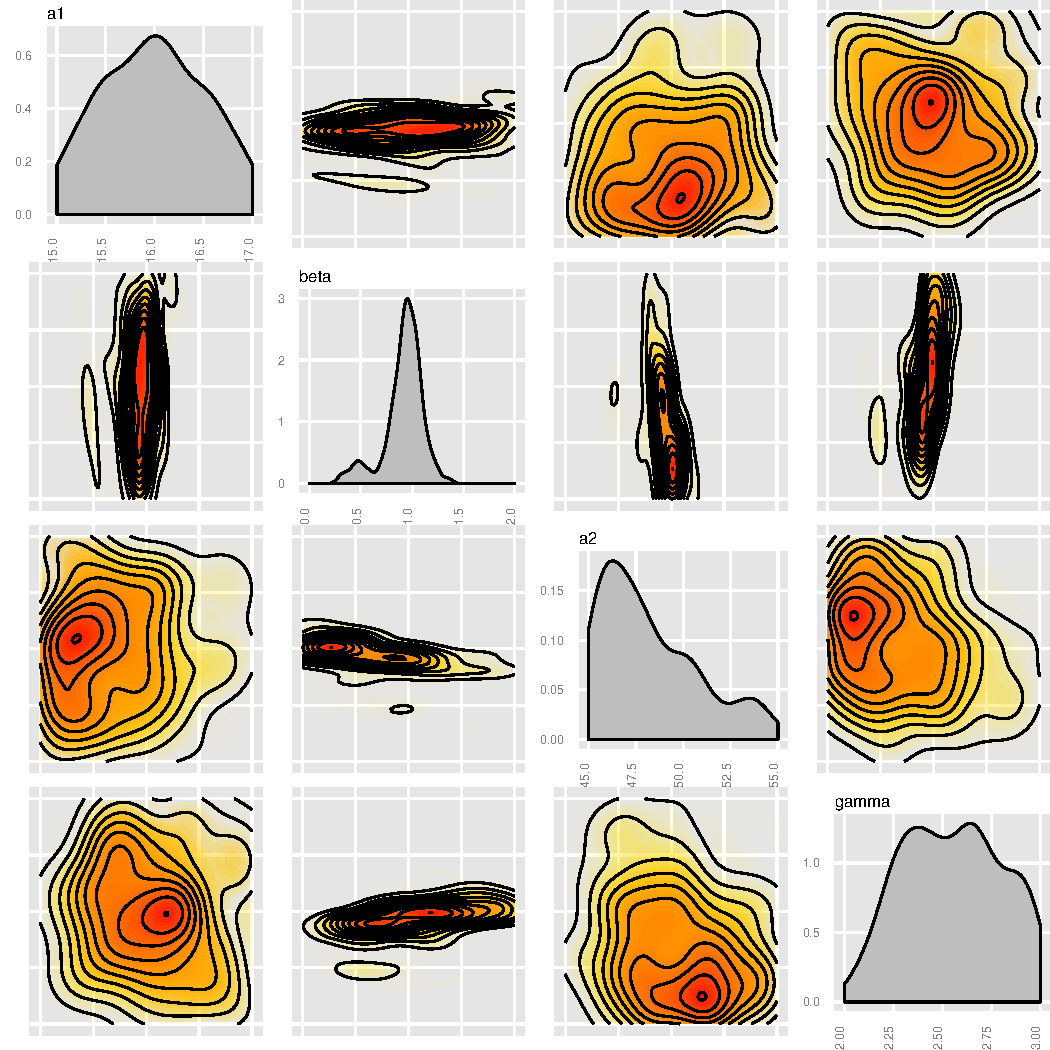
\includegraphics[scale=0.7]{chapterModelling/images/Gardner/Stoch/posterior_100p.pdf}
%\caption{}
%\label{fig:stch_gard}
%\end{figure}
%
%\begin{table}[ht!]
%\centering
%\caption{Munsky-Khammash stochastic switch priors}
%\label{tab:gard_st}
%\begin{tabular}{cccc|cc}
%\multicolumn{4}{c|}{Parameters} & \multicolumn{2}{c}{Species} \\ %\hline
%$a_1$   & $\beta$   & $a_2$   & $\gamma$  &   $s_1$    &       $s_2$   \\
%15-17   &   0-2     &  45-55  &    2-3    &   0-100    &       0-100   
%\end{tabular}
%\end{table}
%
%These values agree with the ones used by the authors to produce a bistable switch.
%
%\begin{figure}[ht!]
%\centering
%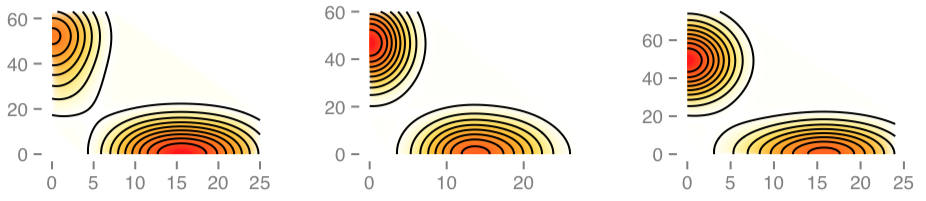
\includegraphics[scale=0.4]{chapterModelling/images/Gardner/Stoch/phase_plots.png}
%\caption{A sample of the phase plots produced from the final population of the Munsky-Khammash switch.}
%\label{fig:stch_gard_phase}
%\end{figure}
%

